\documentclass[UTF8,a4paper,12pt]{ctexart}

\usepackage{geometry}
\usepackage{graphicx}
\usepackage{booktabs}
\usepackage{array}
\usepackage{longtable}
\usepackage{multirow}
\usepackage{amsmath}
\usepackage{xcolor}
\usepackage{float}
\usepackage{caption}
\usepackage{subcaption}
\usepackage{hyperref}
\usepackage{enumitem}

\geometry{left=2.7cm,right=2.7cm,top=2.6cm,bottom=2.6cm}
\hypersetup{
  colorlinks=true,
  linkcolor=blue,
  citecolor=blue,
  urlcolor=blue
}
\emergencystretch=3em
\setlist{nosep}
\captionsetup{font=small,labelfont=bf}

\title{\heiti 基于 Qwen3-8B QLoRA 的中文金融舆情风险智能预警系统}
\author{10225001426\quad 杨巨豪}
\date{\today}

\begin{document}

\maketitle

\begin{abstract}
金融舆情风险常先于正式公告、监管处罚或违约事件出现在新闻、投诉平台和社交媒体中。传统情感分类只能判断文本整体倾向，难以回答风控系统更关心的问题：是否存在风险、风险指向哪个主体、该主体是否需要进入审核流程。围绕中文金融负面主体识别任务，本文基于 FinCUGE-Instruction 中的 FINNSP 数据集，构建数据处理、模型训练、实体抽取、可靠性分析和系统原型相结合的实验方案。模型层面，本文比较 TF-IDF、中文 RoBERTa、MacBERT、FinBERT2-large 与 Qwen3-8B QLoRA 指令微调模型；系统层面，将 \texttt{has\_negative + entities} 扩展为风险事件、风险评分、主体画像和审核队列，并实现 FastAPI 与 Streamlit 演示原型。

实验结果表明，Qwen3-8B QLoRA 主模型在 FINNSP 验证集上取得 Accuracy 0.9720、F1 0.9732、Macro-F1 0.9719、Entity-F1 0.8331，非法 JSON 率为 0。相比最优编码器 FinBERT2-large 的二分类 F1 0.9638，主模型在保持较高分类效果的同时输出负面主体，更符合实体级风险归因需求。离线级联模拟显示，使用 FinBERT2-large 初筛并仅对正例候选调用 Qwen3-8B QLoRA 时，LLM 调用率为 53.2\%，F1 和 Entity-F1 分别为 0.9710、0.8386。外部 FLARE-zh-NSP 二分类评估中，主模型取得 F1 0.9715；反事实压力测试则显示模型在干扰主体和否定语境下较稳，但在主体替换和负面触发词删除上仍有明显边界。结合实体在文率、幻觉实体率、漂移监控和 OpenML 信用违约 tabular 实验，本文给出了一套可复现的中文金融舆情风险预警原型。

\noindent\textbf{关键词：} 金融 NLP；风控预警；负面主体识别；QLoRA；Qwen3；实体归因；舆情监控
\end{abstract}

\newpage
\tableofcontents
\newpage

\section{引言}

在互联网金融、消费信贷、支付、资管和地方金融机构等业务场景中，风险事件通常不会以结构化数据的形式第一时间出现。借款人投诉、投资人维权、媒体报道、监管约谈和平台公告都可能先以非结构化文本形式传播。如果风控系统只能依赖逾期记录、交易流水、征信变量等结构化特征，就可能错过舆情早筛窗口。因此，从中文金融文本中识别负面风险主体，是风控早预警和人工审核分流中的重要任务。

普通情感分类在该问题上存在明显不足。首先，金融文本中的负面表达不一定指向被评估主体。例如监管部门处罚某平台时，监管部门并不是风险主体。其次，一个文本可能包含多个公司、平台或人员，整体情绪为负并不能说明每个主体都有风险。再次，真实风控系统需要把识别结果写入审核队列或主体画像，单纯输出正负标签无法支撑后续处置。因此，本文将任务定义为实体级金融负面主体识别：给定一段金融新闻或社交媒体文本，判断是否存在负面金融风险信息，并抽取被负面信息指向的主体。

本文不只追求单一排行榜指标，而是围绕风控预警构建可复现、可解释、可演示的技术路线。传统机器学习和中文预训练编码器用于建立强基线，并检验数据处理和评价脚本的可靠性；Qwen3-8B QLoRA 指令微调用于统一输出 JSON schema，同时完成二分类和主体抽取；实体候选过滤、风险事件弱标签、风险评分、主体画像、审核队列和模型监控则服务于风控应用。最后，FastAPI 与 Streamlit 原型使模型结果能够进入可交互的审核流程。

本文主要贡献包括：

\begin{enumerate}
  \item 构建统一 JSON schema 的中文金融负面主体识别实验框架，将原始自然语言标签转换为 \texttt{has\_negative} 与 \texttt{entities}，并统一二分类和实体级评估。
  \item 比较传统模型、中文编码器、金融领域编码器和 Qwen3-8B QLoRA 主模型，最终主模型取得 F1 0.9732、Entity-F1 0.8331。
  \item 设计 FinBERT2-large 初筛与 Qwen3-8B QLoRA 复核的离线级联流程，在降低 LLM 调用率的同时保持较高实体级效果。
  \item 将课程任务扩展为风控预警系统原型，包含风险事件、风险评分、主体画像、SQLite 本地库、FastAPI 服务、Streamlit 审核台和漂移监控。
  \item 对模型输出可靠性进行分析，报告实体在文率、幻觉实体率、错误类型和多主体归因问题，并明确区分真实模型评估、弱监督扩展和规则 baseline。
\end{enumerate}

\section{相关工作}

\subsection{通用预训练语言模型与中文编码器}

预训练语言模型已经成为文本分类、信息抽取和语义匹配任务的基础组件。BERT 通过双向 Transformer 编码器和掩码语言模型预训练显著提升了下游自然语言理解效果\cite{bert}；RoBERTa 进一步优化预训练策略、数据规模和训练设置，在多项分类与阅读理解任务中取得更稳定的表现\cite{roberta}。中文场景中，MacBERT 针对中文预训练中的掩码替换策略进行改进，在中文自然语言理解任务上表现突出\cite{macbert}。这些编码器模型的优势是推理速度快、输出稳定、部署成本低，因此适合在金融舆情系统中承担全量初筛角色。

不过，编码器模型通常以 \texttt{[CLS]} 表示接分类头，天然适合输出固定类别，却不能直接生成负面主体列表。若要同时完成风险判断与主体归因，往往还需要额外的命名实体识别、序列标注、实体链接或规则模块。本文保留 TF-IDF、RoBERTa、MacBERT 和 FinBERT2-large 等编码器基线，是为了回答两个问题：其一，课程数据上的二分类强基线能达到什么水平；其二，在风控系统中，轻量模型是否可以作为高吞吐初筛器，与生成式大模型形成互补。

\subsection{金融 NLP 与金融大模型}

金融 NLP 研究长期关注公告分类、情感分析、事件抽取、研报理解、舆情监控和金融问答等任务。与通用领域 NLP 相比，金融文本具有实体密集、术语专业、风险表达隐晦和业务后果敏感等特点。早期金融领域模型通常沿用领域语料预训练加下游分类微调的路线，例如 FinBERT 面向金融情感分析任务验证了领域预训练的价值\cite{finbert}。中文金融场景中，BBT-Fin 与 FinCUGE 等工作推动了金融理解、生成和评测基准建设\cite{bbtfin}，本文使用的 FINNSP 任务来自 FinCUGE-Instruction 数据集\cite{fincuge}。

随着大语言模型发展，金融 NLP 开始从单一分类任务扩展到指令理解、解释生成、多任务问答和工具化系统。BloombergGPT 展示了金融专用大模型在金融任务上的潜力\cite{bloomberggpt}；FinGPT 强调以开源方式构建金融领域大模型与数据工程流程\cite{fingpt}；PIXIU/FinBen 则从多任务基准角度评估金融大模型能力\cite{pixiu}。相关研究提示，金融大模型的价值不只在于分类分数，还在于能否把非结构化文本转换为可被业务流程消费的结构化风险信息。本文的风险事件、主体画像和审核队列设计，与这一思路相一致。

\subsection{实体级风险识别与风控归因}

普通情感分类只判断文本整体倾向，而金融风控更关心实体级归因。比如同一句文本中可能同时出现监管机构、涉事平台、投资人和第三方支付公司，真正需要进入预警名单的通常只是被投诉、被处罚或发生兑付风险的主体。若模型把风险归因到无关主体，会带来误伤；若模型只判断为负面但漏掉主体，则难以写入主体画像和审核队列。因此，负面主体识别比一般情感分类更接近真实风控需求。

FINNSP 与 FLARE-zh-NSP 均可视为中文金融负面主体识别相关任务\cite{fincuge,flare}。本文在任务定义上同时评估二分类指标和 entity-level 指标，并额外统计实体在文率、幻觉实体率和 entity missing review。这种评价方式区别于只报告 Accuracy 或 F1 的分类实验，更强调金融场景中风险判断正确和主体归因正确两个目标必须同时成立。

\subsection{参数高效微调与结构化生成}

大语言模型具备更强的指令理解和结构化生成能力，可以在同一提示词下完成分类、抽取和解释。但直接 zero-shot 或 few-shot 调用大模型存在格式不稳定、实体幻觉和成本较高等问题。LoRA 通过在冻结基座模型参数的前提下训练低秩适配矩阵，显著降低微调参数量\cite{lora}；QLoRA 在此基础上结合 4-bit 量化和低秩适配，使单机多卡环境下微调数十亿参数模型更加可行\cite{qlora}。

本文基于 Qwen3-8B 进行 QLoRA 指令微调，使模型输出受控 JSON，并通过实体候选约束、非法 JSON 兜底解析、幻觉实体标记和人工审核队列降低生成式模型在风控场景中的风险。与只追求端到端生成不同，本文把 LLM 放入可审计的系统流程：编码器负责低成本筛选，LLM 负责高风险样本复核和主体抽取，规则与数据库负责结果校验、沉淀和监控。

\section{数据集与任务定义}

本文主数据集为 FinCUGE-Instruction 中的 FINNSP 任务。该任务来自中文金融负面主体识别场景，训练集包含 4000 条样本，验证集包含 500 条样本。每条样本包含金融文本、任务指令和原始输出。数据处理阶段将原始输出统一转换为 \texttt{has\_negative} 与 \texttt{entities} 两个字段。

数据文本主要来自金融新闻、社交媒体、维权帖、平台公告和行业资讯等非结构化来源，语言风格差异较大。一部分样本类似正式新闻，句式清楚，风险触发词明显，例如涉嫌诈骗、立案侦查、非法吸收公众存款等；另一部分样本来自社交媒体，常包含话题标签、转发符号、URL、乱码、口语化表达和多个无关主体。还有一些负例虽然包含金融产品或平台名称，例如白条、网贷平台数据报告、行业资讯等，但文本并未表达针对该主体的负面风险。这样的数据构成使任务不能被简单理解为关键词匹配：模型既要识别金融风险触发线索，也要判断该线索是否真正指向某个金融主体。

表 \ref{tab:data_examples} 给出若干脱敏与截断后的样例。样例显示，正例可能只有一个风险主体，也可能存在多个风险主体；负例则可能含有金融实体和金融业务词，但不应输出负面主体。本文提交包中仅包含少量脱敏样例文件，不包含全量训练数据。

\begin{table}[H]
\centering
\caption{FINNSP 脱敏样例}
\label{tab:data_examples}
\scriptsize
\setlength{\tabcolsep}{3pt}
\renewcommand{\arraystretch}{1.15}
\begin{tabular}{>{\raggedright\arraybackslash}p{0.13\textwidth}>{\raggedright\arraybackslash}p{0.43\textwidth}>{\centering\arraybackslash}p{0.11\textwidth}>{\raggedright\arraybackslash}p{0.22\textwidth}}
\toprule
样例 & 文本片段 & 负面标签 & 负面主体 \\
\midrule
多主体正例 & \#小资钱包涉嫌诈骗\# 出借受害人期待执法透明，追查相关涉案资产与第三方支付线索…… & true & 小资钱包；北京正聚源通鼎信用管理有限公司 \\
单主体正例 & 重庆市反诈骗中心民警发现疑似诈骗线索：一家名为北银创投的公司涉嫌网络贷款诈骗犯罪。 & true & 北银创投 \\
无负面负例 & 京东白条是先消费后付款的支付方式，可用于京东商城等消费场景，文本为产品介绍和网页噪声…… & false & 空列表 \\
\bottomrule
\end{tabular}
\end{table}

任务包含两个层次。第一层是二分类，即判断文本是否包含针对金融主体的负面风险信息。第二层是主体抽取，即在正例样本中抽取负面风险指向的公司、平台、机构或产品名称。二分类指标包括 Accuracy、Precision、Recall、F1 和 Macro-F1；实体抽取以样本为单位比较 gold 主体集合与预测主体集合，并采用 entity-level Precision、Recall 和 Micro-F1。对于 LLM，还额外统计 invalid JSON rate 和平均推理耗时。

从风控角度看，该任务比普通情感分类更贴近真实应用。情感分类只能判断文本是否整体负面，而负面主体识别能够进一步定位风险指向的主体。后者可以直接进入主体画像、风险名单、人工审核队列和后续反欺诈线索分析。

\begin{figure}[H]
  \centering
  \begin{subfigure}{0.48\textwidth}
    \centering
    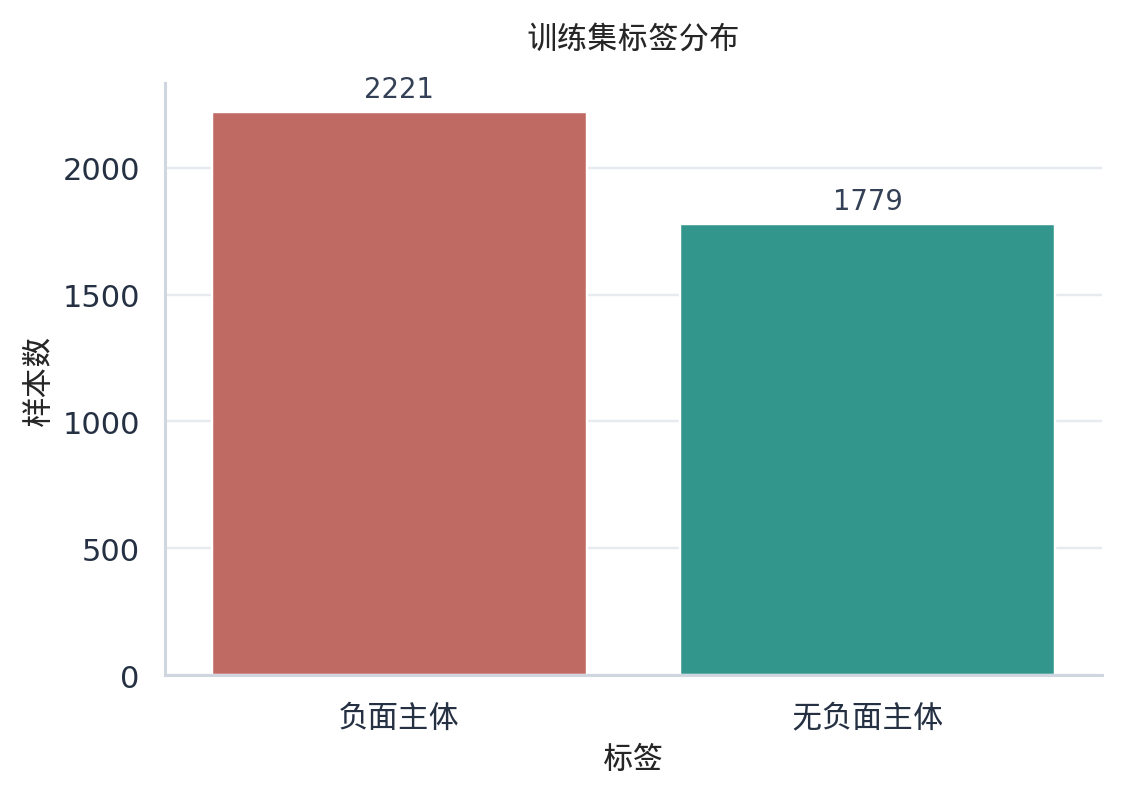
\includegraphics[width=\linewidth]{../outputs/figures/train_label_distribution.png}
    \caption{训练集标签分布}
  \end{subfigure}
  \hfill
  \begin{subfigure}{0.48\textwidth}
    \centering
    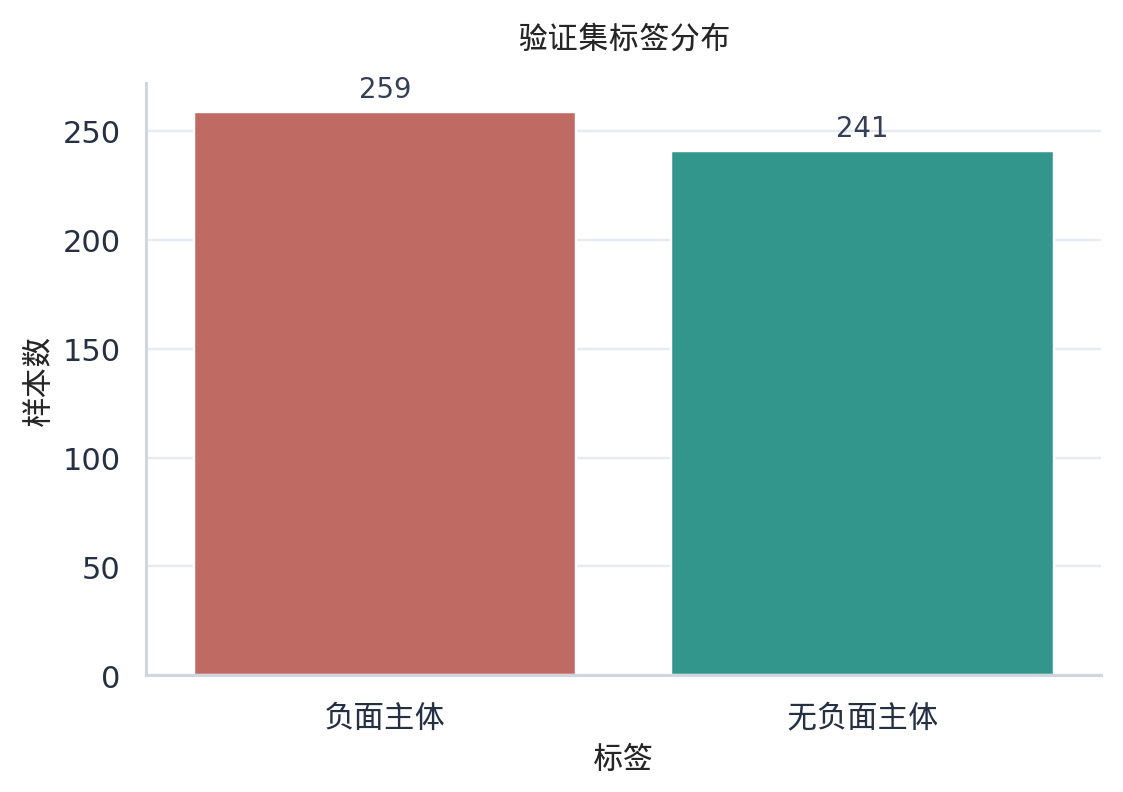
\includegraphics[width=\linewidth]{../outputs/figures/eval_label_distribution.png}
    \caption{验证集标签分布}
  \end{subfigure}
  \caption{FINNSP 标签分布}
  \label{fig:label_distribution}
\end{figure}

\begin{figure}[H]
  \centering
  \begin{subfigure}{0.48\textwidth}
    \centering
    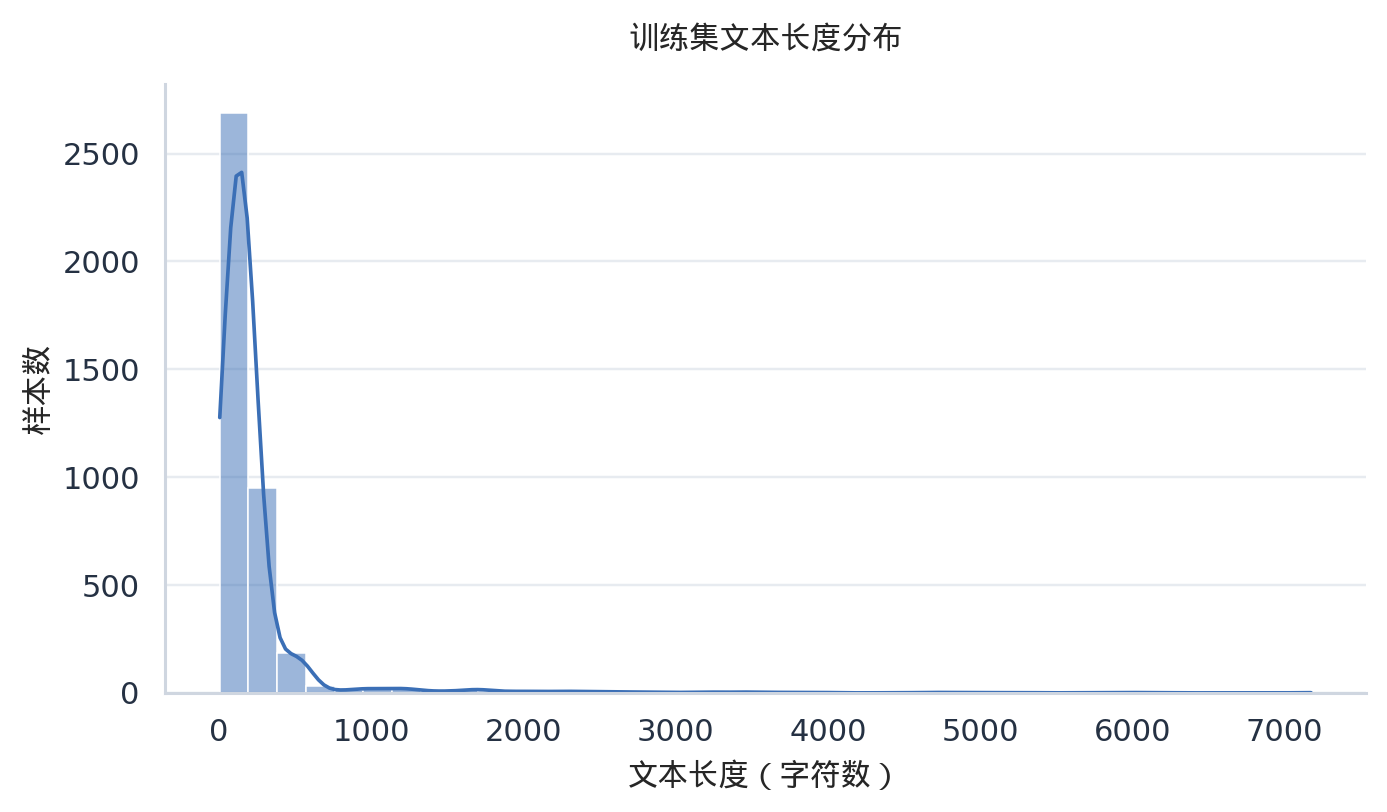
\includegraphics[width=\linewidth]{../outputs/figures/train_text_length_distribution.png}
    \caption{训练集文本长度}
  \end{subfigure}
  \hfill
  \begin{subfigure}{0.48\textwidth}
    \centering
    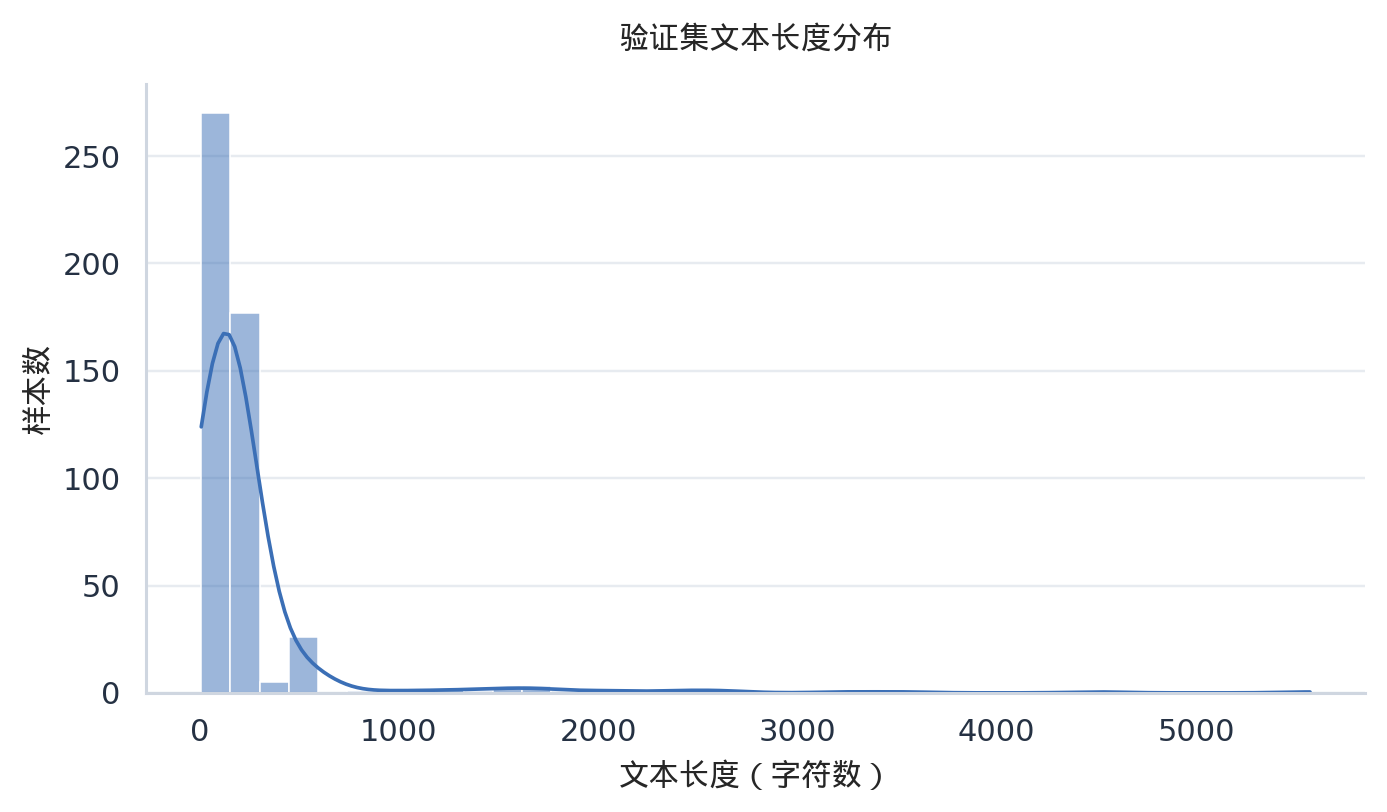
\includegraphics[width=\linewidth]{../outputs/figures/eval_text_length_distribution.png}
    \caption{验证集文本长度}
  \end{subfigure}
  \caption{FINNSP 文本长度分布}
  \label{fig:length_distribution}
\end{figure}

\section{方法}

整体方法如图 \ref{fig:system_framework} 所示。数据层负责对金融新闻、公告、投诉和社交媒体文本进行清洗、脱敏、标签归一化与实体候选构造；模型层以编码器模型完成高吞吐初筛，并使用 Qwen3-8B QLoRA 对高风险文本进行复核和主体抽取；业务层将结构化输出写入风险事件库、主体画像、审核队列和监控模块。该框架强调模型结果在风控链路中的可消费性，而不只停留在离线分类分数。

\begin{figure}[H]
  \centering
  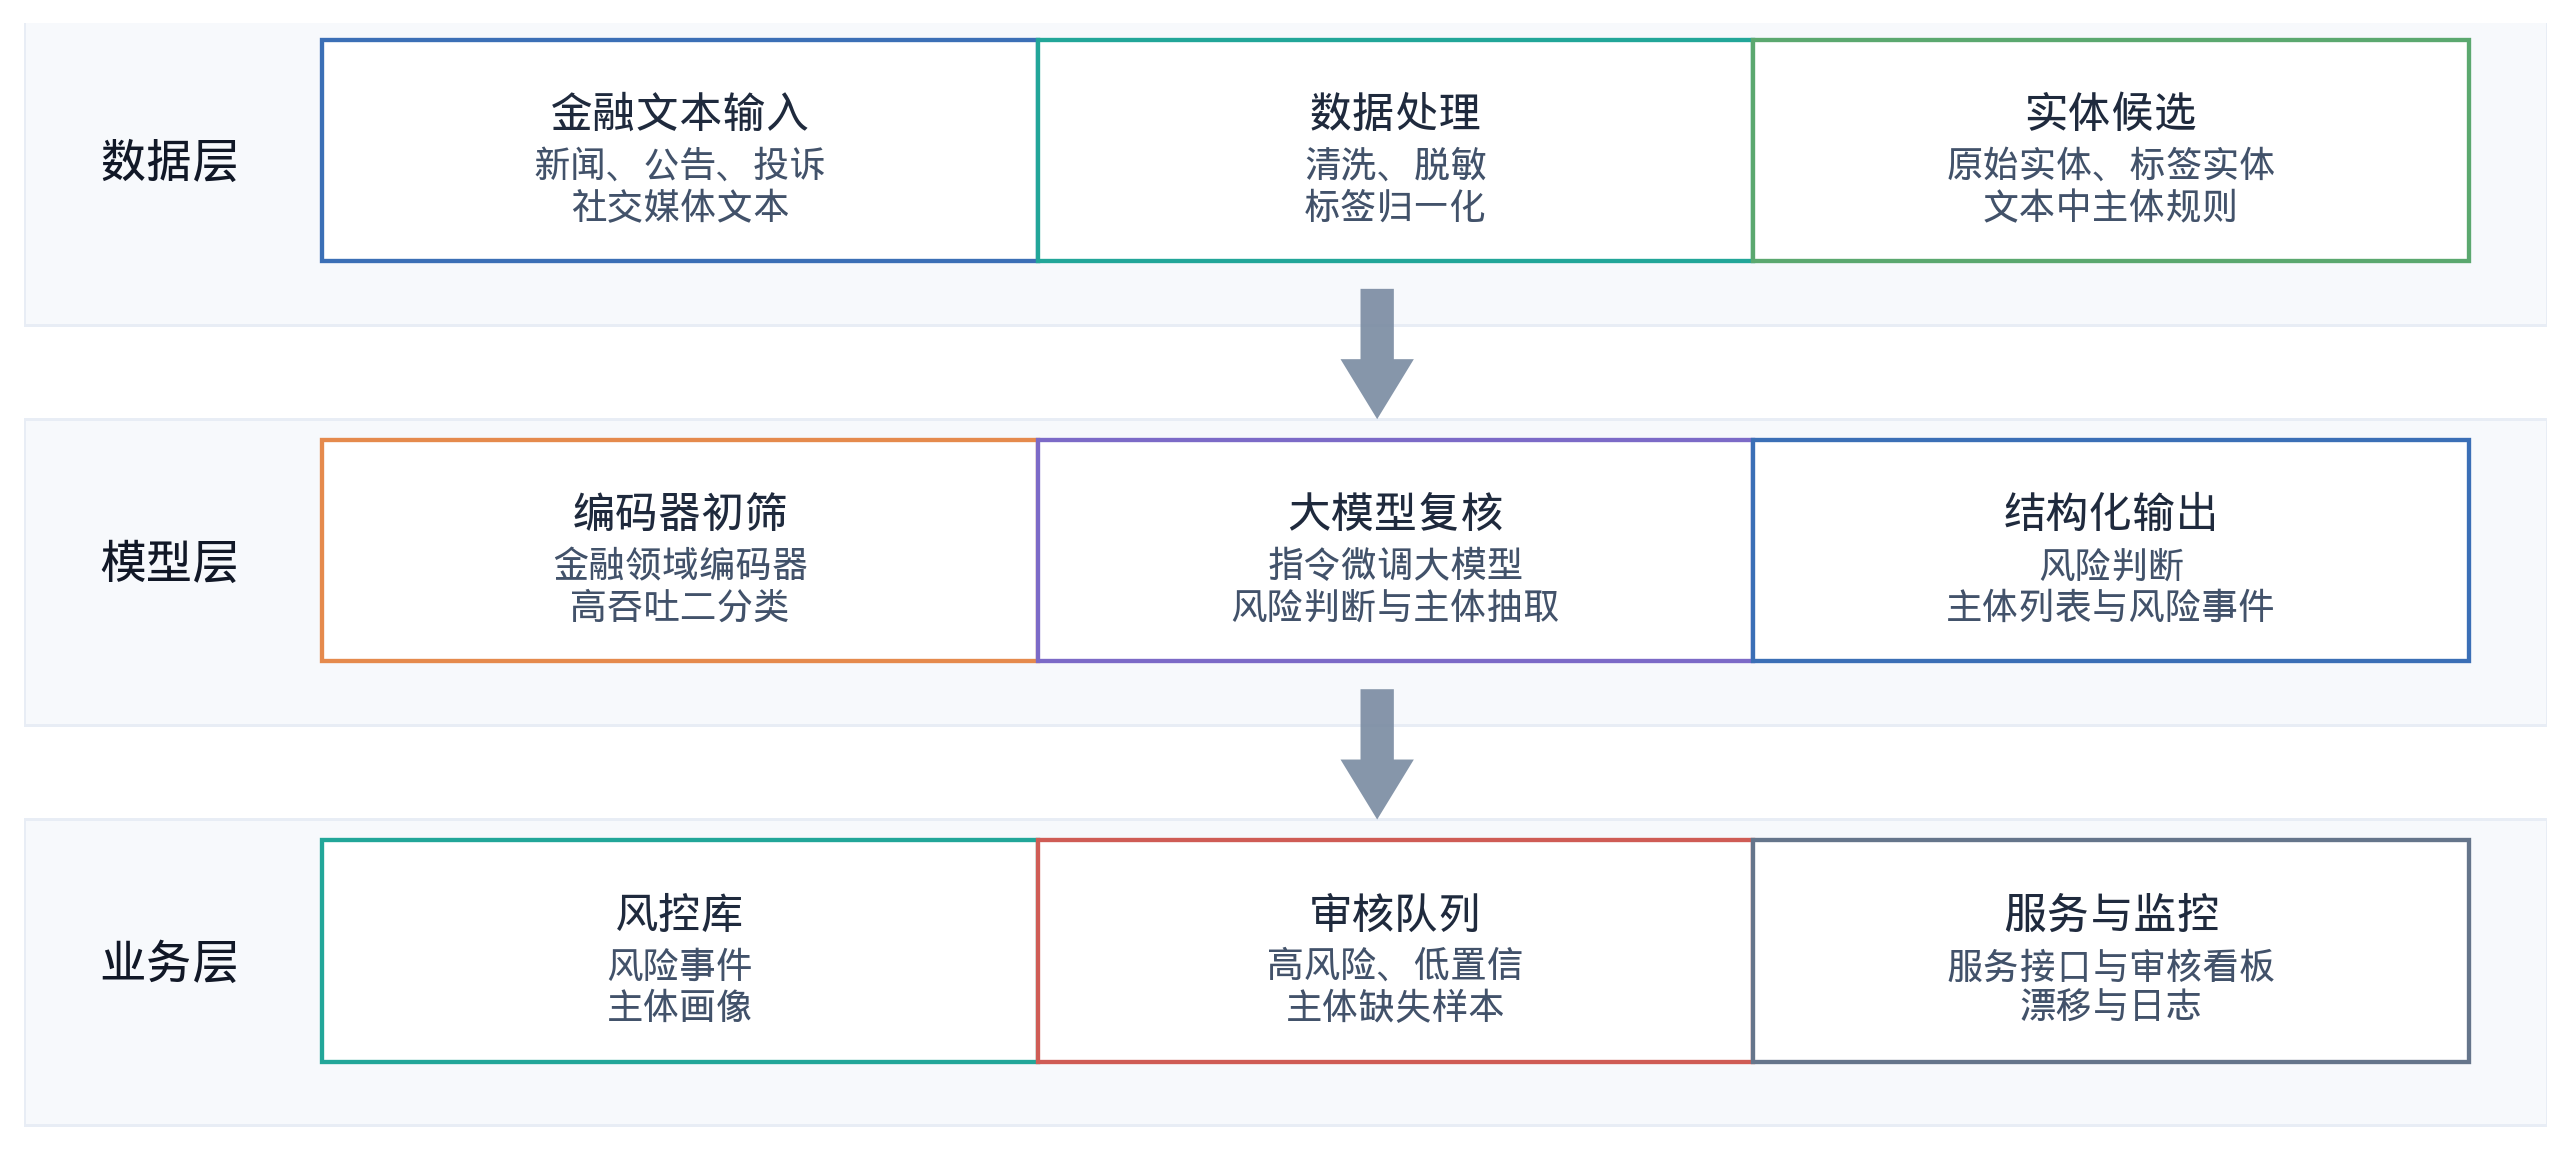
\includegraphics[width=0.96\textwidth]{../outputs/figures/system_framework.png}
  \caption{中文金融舆情风险智能预警系统总体框架}
  \label{fig:system_framework}
\end{figure}

\subsection{传统基线}

传统基线使用 TF-IDF 表示文本，并分别训练 Logistic Regression 与 Linear SVM。该组实验训练速度快、可解释性强，用于验证数据切分和评价脚本是否正确。虽然 TF-IDF 无法深层理解上下文，但在金融负面词明显的文本中仍能取得较强二分类效果。

具体实现上，本文采用字符级 2--4 gram TF-IDF 特征。选择字符级特征而不是先分词，是因为数据中包含平台简称、公司名、话题标签、URL 和口语化片段，字符 n-gram 对中文未登录词和噪声文本更稳健。设 $g_j$ 表示第 $j$ 个字符 n-gram，$N$ 为训练语料文档数，$\mathrm{df}(g_j)$ 为包含该 n-gram 的文档数，则文本 $x$ 的第 $j$ 维特征和线性分类得分可写为式 \ref{eq:tfidf_linear}。

\begin{equation}
\begin{aligned}
v_j(x)&=\mathrm{tf}(g_j,x)\log\frac{N+1}{\mathrm{df}(g_j)+1},\\
f(x)&=w^\top v(x)+b,\quad p(y=1\mid x)=\sigma(f(x)).
\end{aligned}
\label{eq:tfidf_linear}
\end{equation}

Logistic Regression 直接使用 $\sigma(f(x))$ 得到正例概率，Linear SVM 则使用同一类稀疏特征学习最大间隔分类超平面。二者均使用类别权重缓解正负样本比例差异，最终只输出二分类标签，不输出主体列表。因此，这组模型主要用于提供传统 NLP 基线，并检验关键词线索在该任务中的强度。

\subsection{中文编码器模型}

编码器模型包括 Chinese RoBERTa-wwm-ext、Chinese MacBERT-base 和 FinBERT2-large。这类模型以 \texttt{[CLS]} 表示接分类头，主要用于二分类。FinBERT2-large 是金融领域模型，适合承担线上高吞吐初筛职责。其局限是不能直接生成主体列表，因此 Entity-F1 为 0。

编码器训练时将文本截断到固定长度，输入 Transformer 编码器后取句级表示接二分类线性层，使用交叉熵损失优化无负面/有负面标签。其核心计算如式 \ref{eq:encoder_classifier} 所示，其中 $h_{\mathrm{cls}}$ 为 \texttt{[CLS]} 位置的上下文表示，$W_c$ 和 $b_c$ 为下游分类头参数。

\begin{equation}
h_{\mathrm{cls}}=\mathrm{Encoder}_{\theta}(x)_{\mathrm{cls}},\quad
p(y\mid x)=\mathrm{softmax}(W_ch_{\mathrm{cls}}+b_c).
\label{eq:encoder_classifier}
\end{equation}

RoBERTa 与 MacBERT 代表通用中文预训练模型，FinBERT2-large 代表金融领域预训练模型。三者与传统 TF-IDF 基线形成由浅到深的对照：若编码器显著优于 TF-IDF，说明模型确实利用了上下文语义；若金融领域编码器优于通用编码器，则说明领域预训练对金融舆情文本有帮助。

\subsection{大模型指令微调动机}

本文将不含标注示例、只给任务说明和输出格式要求的设置称为 zero-shot；将少量训练样例及其标准 JSON 输出拼接到提示词中的设置称为 few-shot。二者都不更新模型参数，主要用于评估通用大模型在无训练或少量示例条件下的直接迁移能力。

在前期探索中，直接使用大模型进行 zero-shot 或 few-shot 结构化抽取时，虽然能够理解任务，但容易扩大风险主体范围，并在多主体文本中产生实体误报。金融风控系统要求输出字段稳定、实体可追溯、异常可记录，因此本文选择对 Qwen3-8B 进行 QLoRA 指令微调，让模型在统一提示词下稳定输出 \texttt{has\_negative} 与 \texttt{entities}。

\subsection{Qwen3-8B QLoRA 主模型}

主模型基于 Qwen3-8B，采用 4-bit QLoRA 进行参数高效指令微调。训练时冻结基座模型的大部分参数，只更新低秩适配器参数，从而在有限显存条件下完成大模型适配。相比直接使用 zero-shot 提示，QLoRA 微调的目标是让模型学习稳定的任务格式、负面主体归因方式和 JSON 输出约束。

主模型将原始样本组织为系统角色提示、用户任务提示和标准 JSON 答案组成的监督微调样本。系统提示限定模型身份为金融风控文本分析助手，并要求不要输出思考过程、解释文字或 Markdown；用户提示包含待判断文本、字段定义和输出示例；答案为归一化后的 \texttt{\{"has\_negative": bool, "entities": list[str]\}}。训练时，提示词部分的标签被 mask，只在答案 JSON token 上计算自回归语言模型损失，使模型学习在给定文本后生成合法结构化结果。设输入提示为 $x$，标准答案 token 序列为 $y_{1:T}$，mask 变量 $m_t$ 仅在答案 JSON 部分取 1，则监督微调目标可写为式 \ref{eq:sft_loss}。

\begin{equation}
\mathcal{L}_{\mathrm{SFT}}
=-\sum_{t=1}^{T} m_t \log p_{\theta}(y_t \mid x,y_{<t}).
\label{eq:sft_loss}
\end{equation}

QLoRA 部分采用 4-bit NF4 量化加载基座模型，并在 attention 与 MLP 投影层加入 LoRA 适配器。对某个输入维度为 $d$、输出维度为 $k$ 的线性层而言，冻结后的量化基座权重记为 $Q_4(W_0)$，LoRA 只训练低秩矩阵 $A$ 与 $B$，其前向计算如式 \ref{eq:lora_update} 所示，其中 $r$ 为低秩维度，$\alpha$ 为缩放系数。

\begin{equation}
h = Q_4(W_0)x+\Delta Wx,\quad
\Delta W=\frac{\alpha}{r}BA,\quad r\ll \min(d,k).
\label{eq:lora_update}
\end{equation}

该设置保留 Qwen3-8B 的主体知识和语言能力，只通过少量适配器参数完成任务对齐。与完整微调相比，QLoRA 降低了显存占用；与单纯提示相比，它能将只输出 JSON、避免无关主体泛化、负例实体列表为空等格式和任务习惯固化到模型参数中。

推理时采用贪心解码，并关闭 Qwen3 的 thinking 输出，避免 \texttt{<think>} 内容干扰 JSON 解析。若 LLM 输出非法 JSON，解析程序会记录异常并尝试从文本中兜底抽取 \texttt{has\_negative} 和实体列表。最终主模型在验证集上 invalid JSON rate 为 0，表明当前提示与指令微调后的格式约束较稳定。训练、评估和指标计算程序已随提交代码提供，以保证实验可复现。

\subsection{风控事件与系统扩展}

为贴近风控系统，项目将模型输出扩展为风险事件，字段包括主体、风险类型、严重程度、置信度、风险分数、风险等级、证据片段和处置动作。风险类型包括诈骗/非法集资、兑付/逾期风险、监管/处罚风险、经营异常、财务恶化、投诉纠纷、洗钱/涉黑等严重违法。风险类型和严重程度来自关键词弱标注与规则映射，并非人工标注的多分类任务。因此，相关结果只作为风控扩展弱标签分析，不作为真实人工多分类评测。

风险分数采用规则化加权方式计算，如式 \ref{eq:risk_score} 所示。其中 $c_m$ 表示模型置信度，$s_v$ 表示严重程度得分，$s_{\mathrm{src}}$ 表示来源可靠性，$h_e$ 表示主体历史风险得分，$r_t$ 表示时效性得分，各分量均归一化到 $[0,1]$。最终分数映射到 $[0,100]$，再按阈值划分为 low、medium、high 和 critical。

\begin{equation}
\begin{aligned}
S_{\mathrm{risk}}=100(&0.35c_m+0.25s_v+0.20s_{\mathrm{src}}\\
&+0.10h_e+0.10r_t).
\end{aligned}
\label{eq:risk_score}
\end{equation}

\section{实验设置与结果分析}

\subsection{实验设置}

实验环境为 8 张 NVIDIA RTX 3090，主要依赖包括 PyTorch、Transformers、Datasets、PEFT、BitsAndBytes、TRL、scikit-learn、LightGBM、FastAPI 和 Streamlit。所有模型使用相同训练/验证切分，指标由统一评估程序计算。LLM 评估保存预测文件和指标文件，便于后续错误分析和级联模拟。

\subsection{主任务结果}

主任务结果如表 \ref{tab:main_results} 所示。

\begin{table}[H]
\centering
\caption{FINNSP 主任务模型对比结果}
\label{tab:main_results}
\small
\begin{tabular}{lrrrrrr}
\toprule
模型 & Acc. & Prec. & Recall & F1 & Macro-F1 & Entity-F1 \\
\midrule
TF-IDF + LR & 0.9300 & 0.9242 & 0.9421 & 0.9331 & 0.9299 & 0.0000 \\
TF-IDF + SVM & 0.9500 & 0.9432 & 0.9614 & 0.9522 & 0.9499 & 0.0000 \\
Chinese RoBERTa & 0.9540 & 0.9538 & 0.9575 & 0.9557 & 0.9539 & 0.0000 \\
Chinese MacBERT & 0.9580 & 0.9542 & 0.9653 & 0.9597 & 0.9579 & 0.0000 \\
FinBERT2-large & 0.9620 & 0.9511 & 0.9768 & 0.9638 & 0.9619 & 0.0000 \\
Qwen3-8B zero-shot & 0.9060 & 0.8605 & 0.9768 & 0.9150 & 0.9049 & 0.5526 \\
Qwen3-8B few-shot & 0.9340 & 0.8979 & 0.9846 & 0.9392 & 0.9335 & 0.6273 \\
\textbf{Qwen3-8B QLoRA} & \textbf{0.9720} & \textbf{0.9658} & \textbf{0.9807} & \textbf{0.9732} & \textbf{0.9719} & \textbf{0.8331} \\
\bottomrule
\end{tabular}
\end{table}

结果表明，传统机器学习方法已经取得较高二分类效果，FINNSP 文本中确实存在较明显的金融负面线索。中文编码器进一步提升了语义理解能力，其中 FinBERT2-large 达到 F1 0.9638，是最强编码器基线。关闭 thinking 后，Qwen3-8B zero-shot 能够稳定输出合法 JSON，并取得 F1 0.9150；加入 4 个标注示例后，few-shot 进一步提升到 F1 0.9392 和 Entity-F1 0.6273。但二者的 Precision 和 Entity-F1 仍明显低于 QLoRA 主模型，说明未微调大模型更容易扩大风险主体范围并产生实体误报。Qwen3-8B QLoRA 在二分类和实体抽取上取得综合最优效果，表明指令微调对主体归因和误报控制有直接作用。

\begin{figure}[H]
  \centering
  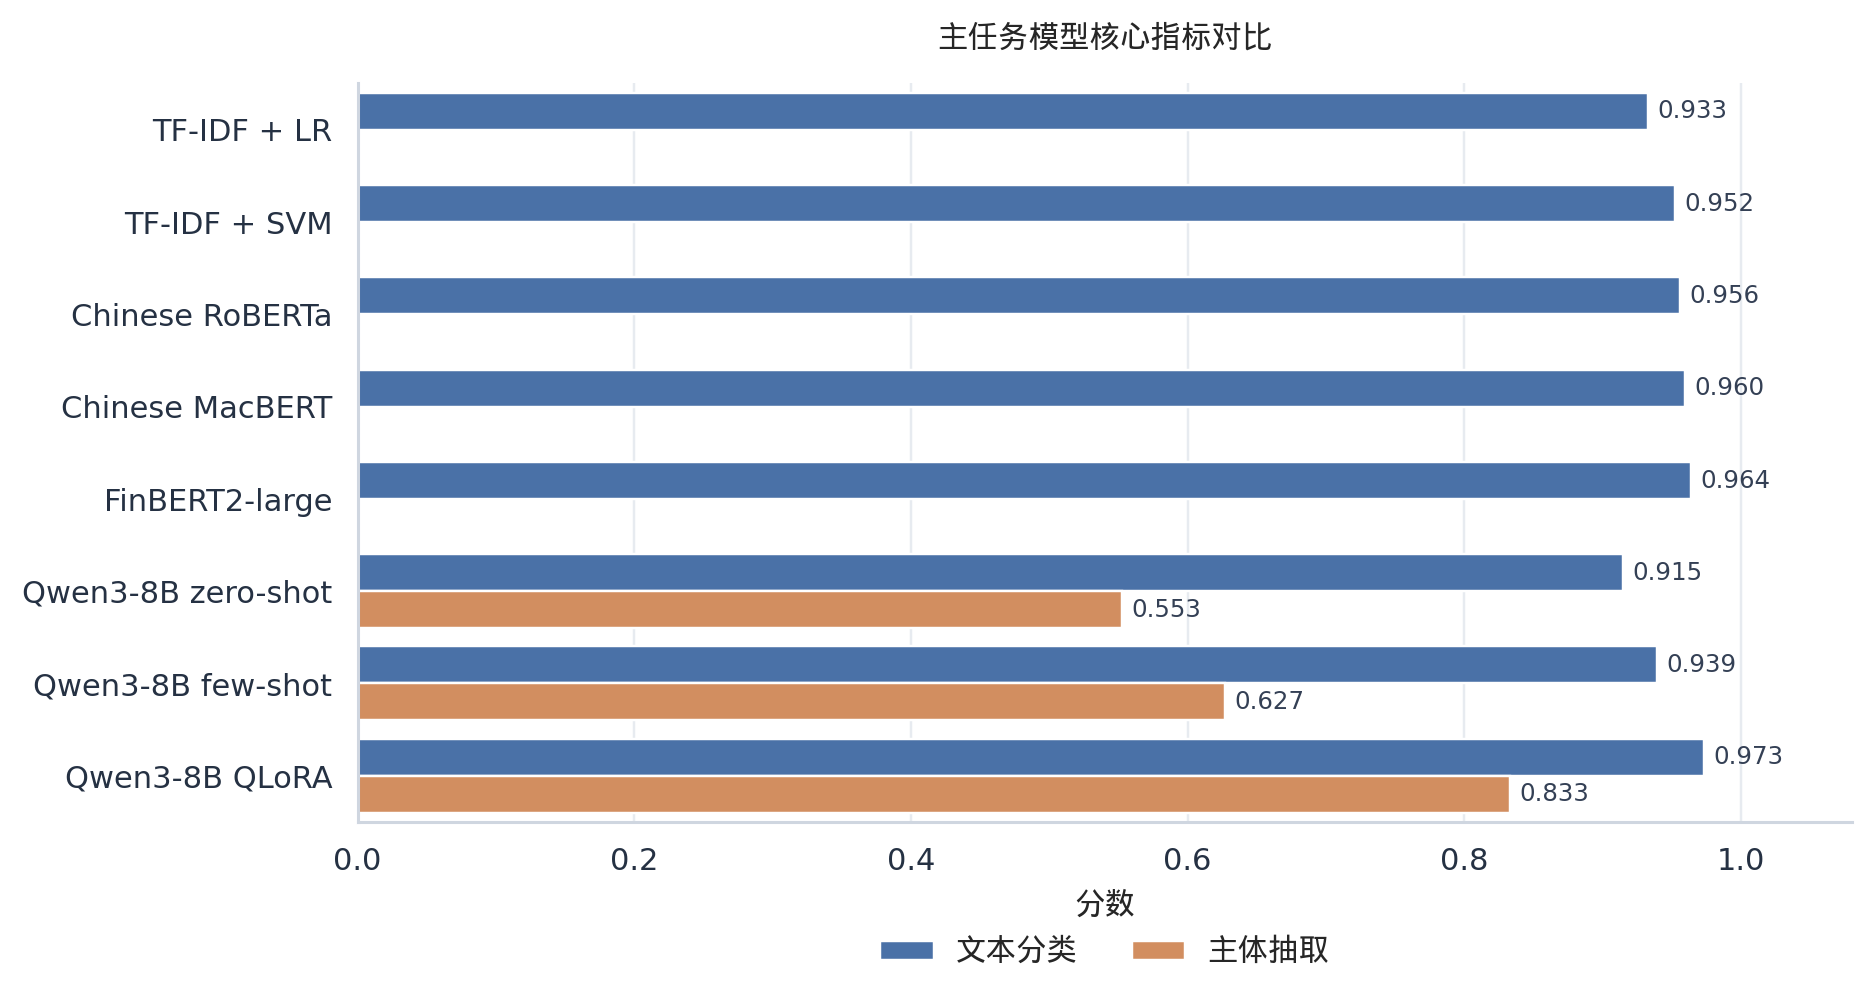
\includegraphics[width=0.86\textwidth]{../outputs/figures/model_comparison_core_metrics.png}
  \caption{主任务模型核心指标对比}
  \label{fig:model_comparison}
\end{figure}

\begin{figure}[H]
  \centering
  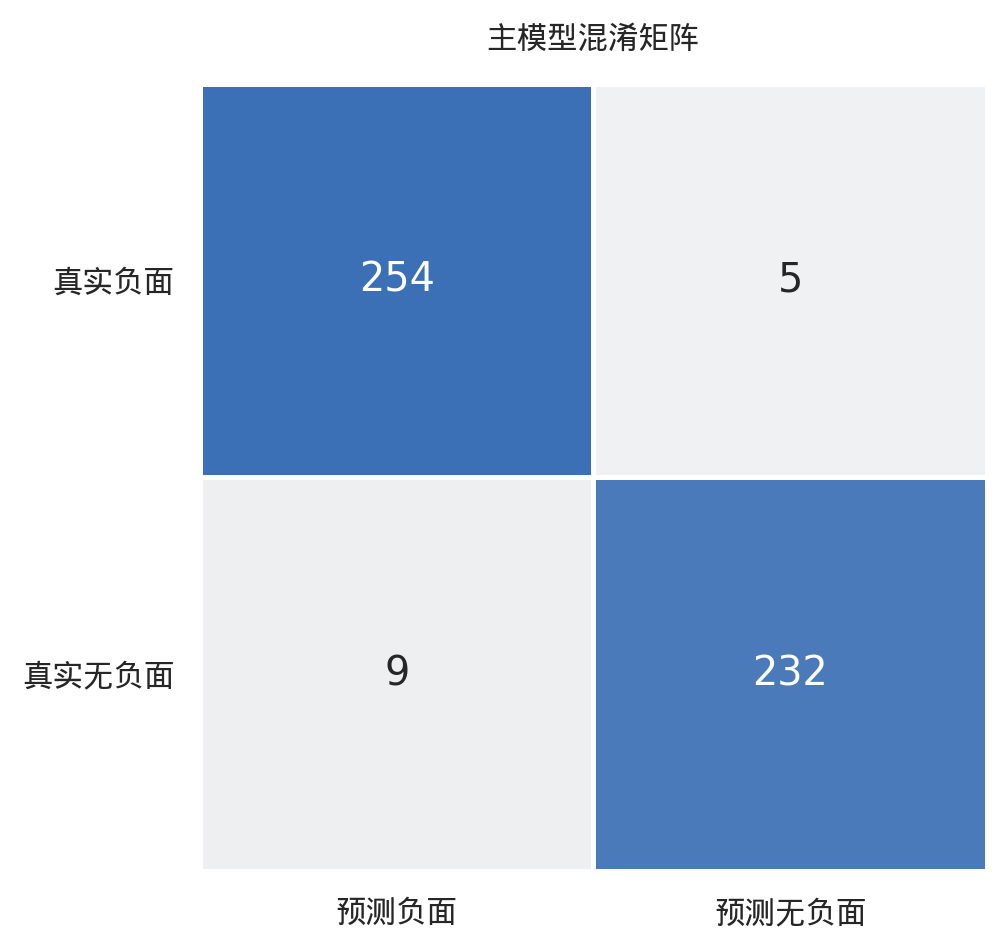
\includegraphics[width=0.72\textwidth]{../outputs/figures/confusion_matrix.png}
  \caption{主模型混淆矩阵}
  \label{fig:confusion_matrix}
\end{figure}

从风控应用角度看，编码器模型适合线上全量初筛，而 QLoRA 模型更适合高风险样本复核。单纯比较 F1 并不能完全体现 LLM 价值，实体级输出、格式稳定性、证据片段和审核队列才是大模型在风控系统中更重要的落点。

\subsection{可靠性与错误分析}

金融风控系统对错误类型较为敏感。False Negative 意味着高风险事件漏报，可能错过预警窗口；False Positive 会增加人工审核成本；Entity Mismatch 可能把风险错误归因给无关主体，造成误伤；Hallucinated Entity 则说明 LLM 输出了原文中不存在的主体，需要上线前规则拦截。

\begin{table}[H]
\centering
\caption{Qwen3-8B QLoRA 可靠性指标}
\label{tab:reliability}
\begin{tabular}{lr}
\toprule
指标 & 数值 \\
\midrule
Invalid JSON rate & 0.0000 \\
预测实体总数 & 441 \\
实体在文数 & 435 \\
实体在文率 & 0.9864 \\
幻觉实体率 & 0.0136 \\
False Positive & 9 \\
False Negative & 5 \\
Entity Mismatch & 72 \\
多主体样本数 & 158 \\
\bottomrule
\end{tabular}
\end{table}

主要错误集中在多主体归因和主体边界不一致。例如文本中同时出现平台、关联公司、监管机构和投资人组织时，模型可能抽取过宽，也可能漏掉某个风险主体。另一个常见问题是简称和全称不一致，例如文本中出现平台简称，而标签使用公司全称，导致实体级评估较严。对于真实风控系统，这类问题可以通过实体链接、别名库和金融 NER 模型进一步缓解。

\subsection{编码器到 LLM 的级联风控模拟}

直接对所有文本调用 LLM 成本较高，也不符合高吞吐风控系统的部署习惯。本文设计离线级联策略：第一阶段使用 FinBERT2-large 判断文本是否有风险；若编码器判断为无风险，则直接放行；若判断为有风险，则调用 Qwen3-8B QLoRA 复核并抽取主体。

\begin{table}[H]
\centering
\caption{FinBERT2 到 Qwen3-8B QLoRA 的离线级联模拟结果}
\label{tab:cascade}
\small
\begin{tabular}{>{\raggedright\arraybackslash}p{4.8cm}rrrrr}
\toprule
设置 & Accuracy & Recall & F1 & Entity-F1 & LLM 调用率 \\
\midrule
FinBERT2 only & 0.9620 & 0.9768 & 0.9638 & 0.0000 & 0.0000 \\
Qwen3-8B QLoRA all & 0.9720 & 0.9807 & 0.9732 & 0.8331 & 1.0000 \\
FinBERT2 positive $\rightarrow$ Qwen3-8B QLoRA & 0.9700 & 0.9691 & 0.9710 & 0.8386 & 0.5320 \\
\bottomrule
\end{tabular}
\end{table}

表中可见，在只调用 53.2\% LLM 的情况下，级联策略仍能保持接近全量 LLM 的二分类 F1，并将 Entity-F1 提升到 0.8386。主要原因是编码器放行了大量负例文本，减少了 LLM 在负例上误抽实体的机会。该实验基于保存预测文件进行离线模拟，不等同于线上真实延迟收益；若要部署到生产环境，还需要评估模型加载、批处理、队列延迟、GPU 利用率和服务稳定性。

\section{风控系统扩展与应用讨论}

\subsection{风控系统原型}

项目实现了本地风控预警系统原型。FastAPI 服务提供 \texttt{/score}、\texttt{/batch\_score}、\texttt{/entity/\{name\}}、\texttt{/review\_queue} 和 \texttt{/metrics} 接口。其中 \texttt{/score} 接收单条文本，执行编码器初筛和 Qwen3 复核，输出风险事件、风险分数和审核标记。SQLite 数据库存储风险事件、主体画像、审核队列、预测日志和漂移快照。Streamlit 审核台展示文本输入、风险识别结果、主体画像、审核队列和服务指标。

系统输出中新增三个风控审核字段：
\begin{itemize}
  \item \texttt{model\_has\_negative}：模型层面是否判断文本存在风险；
  \item \texttt{entity\_missing\_review}：模型判有风险但主体缺失或被过滤时触发人工复核；
  \item \texttt{hallucinated\_entity}：LLM 输出主体被实体候选约束过滤时置为真。
\end{itemize}
当模型判断存在风险但主体不可用时，系统不会自动放行，而是将样本写入审核队列。这一设计符合风控业务逻辑：模型层面的风险判断和实体可用性应分开处理，不能因为主体抽取失败就忽略潜在风险。

\begin{figure}[H]
  \centering
  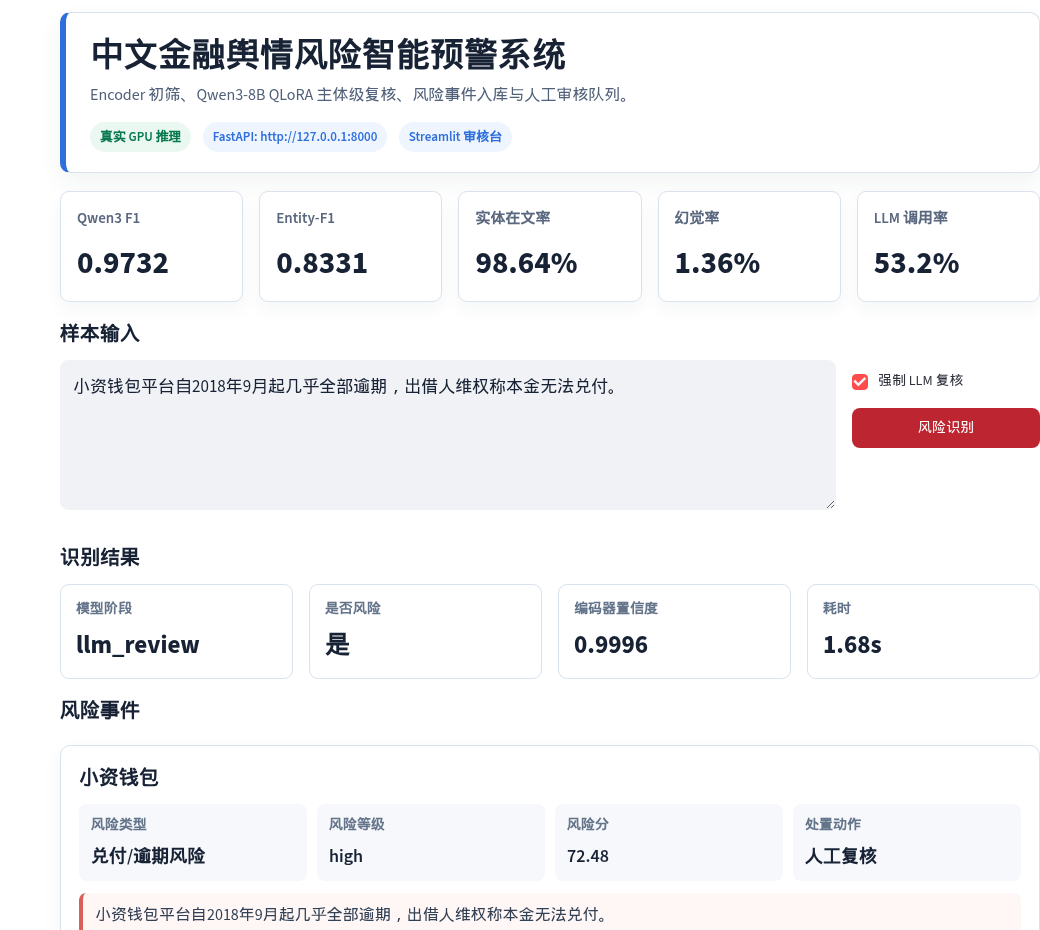
\includegraphics[width=0.95\textwidth]{../outputs/demo_screenshots/streamlit_dashboard_home.png}
  \caption{金融舆情风险审核台真实运行截图}
  \label{fig:demo_dashboard}
\end{figure}

\begin{figure}[H]
  \centering
  \begin{subfigure}{0.92\textwidth}
    \centering
    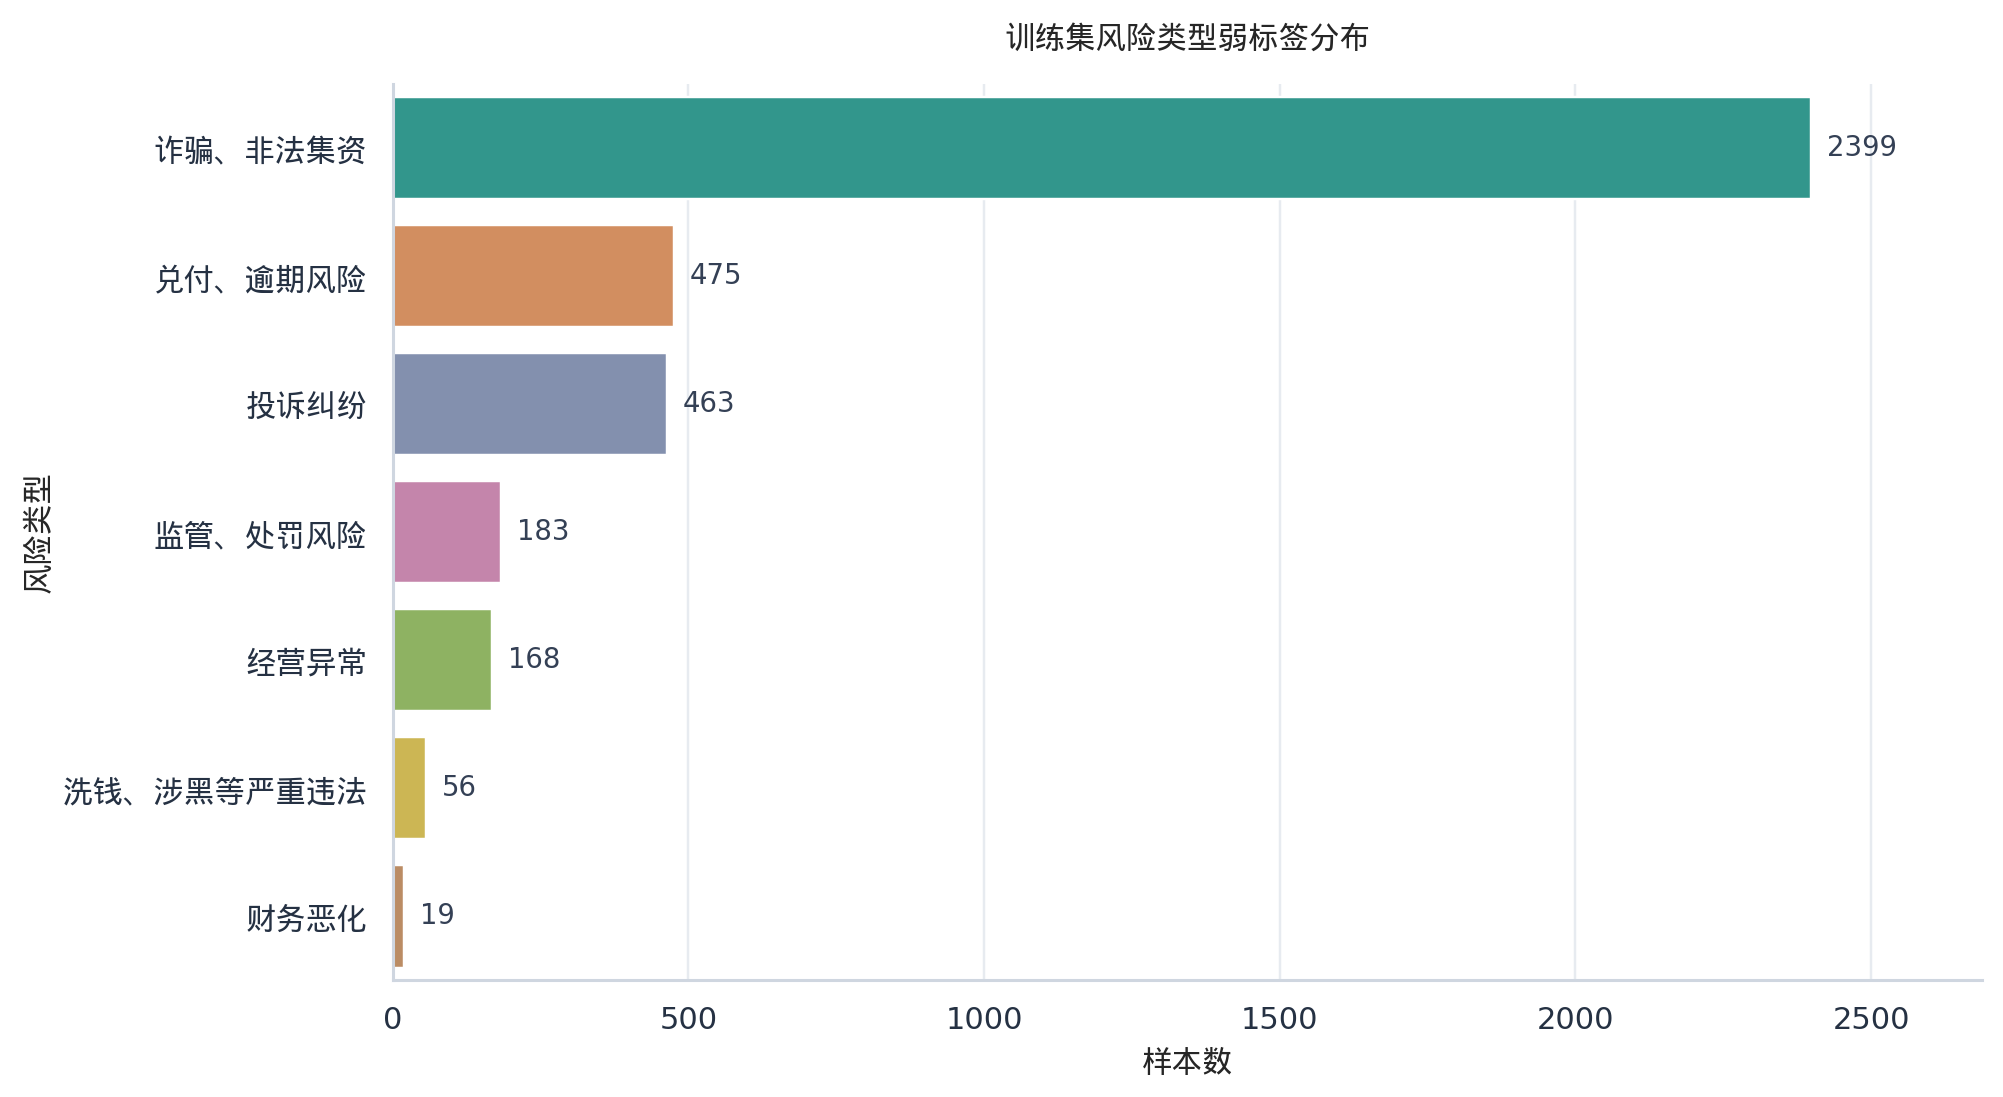
\includegraphics[width=\linewidth]{../outputs/figures/train_risk_type_distribution.png}
    \caption{训练集风险类型弱标签}
  \end{subfigure}
  \vspace{0.8em}
  \begin{subfigure}{0.92\textwidth}
    \centering
    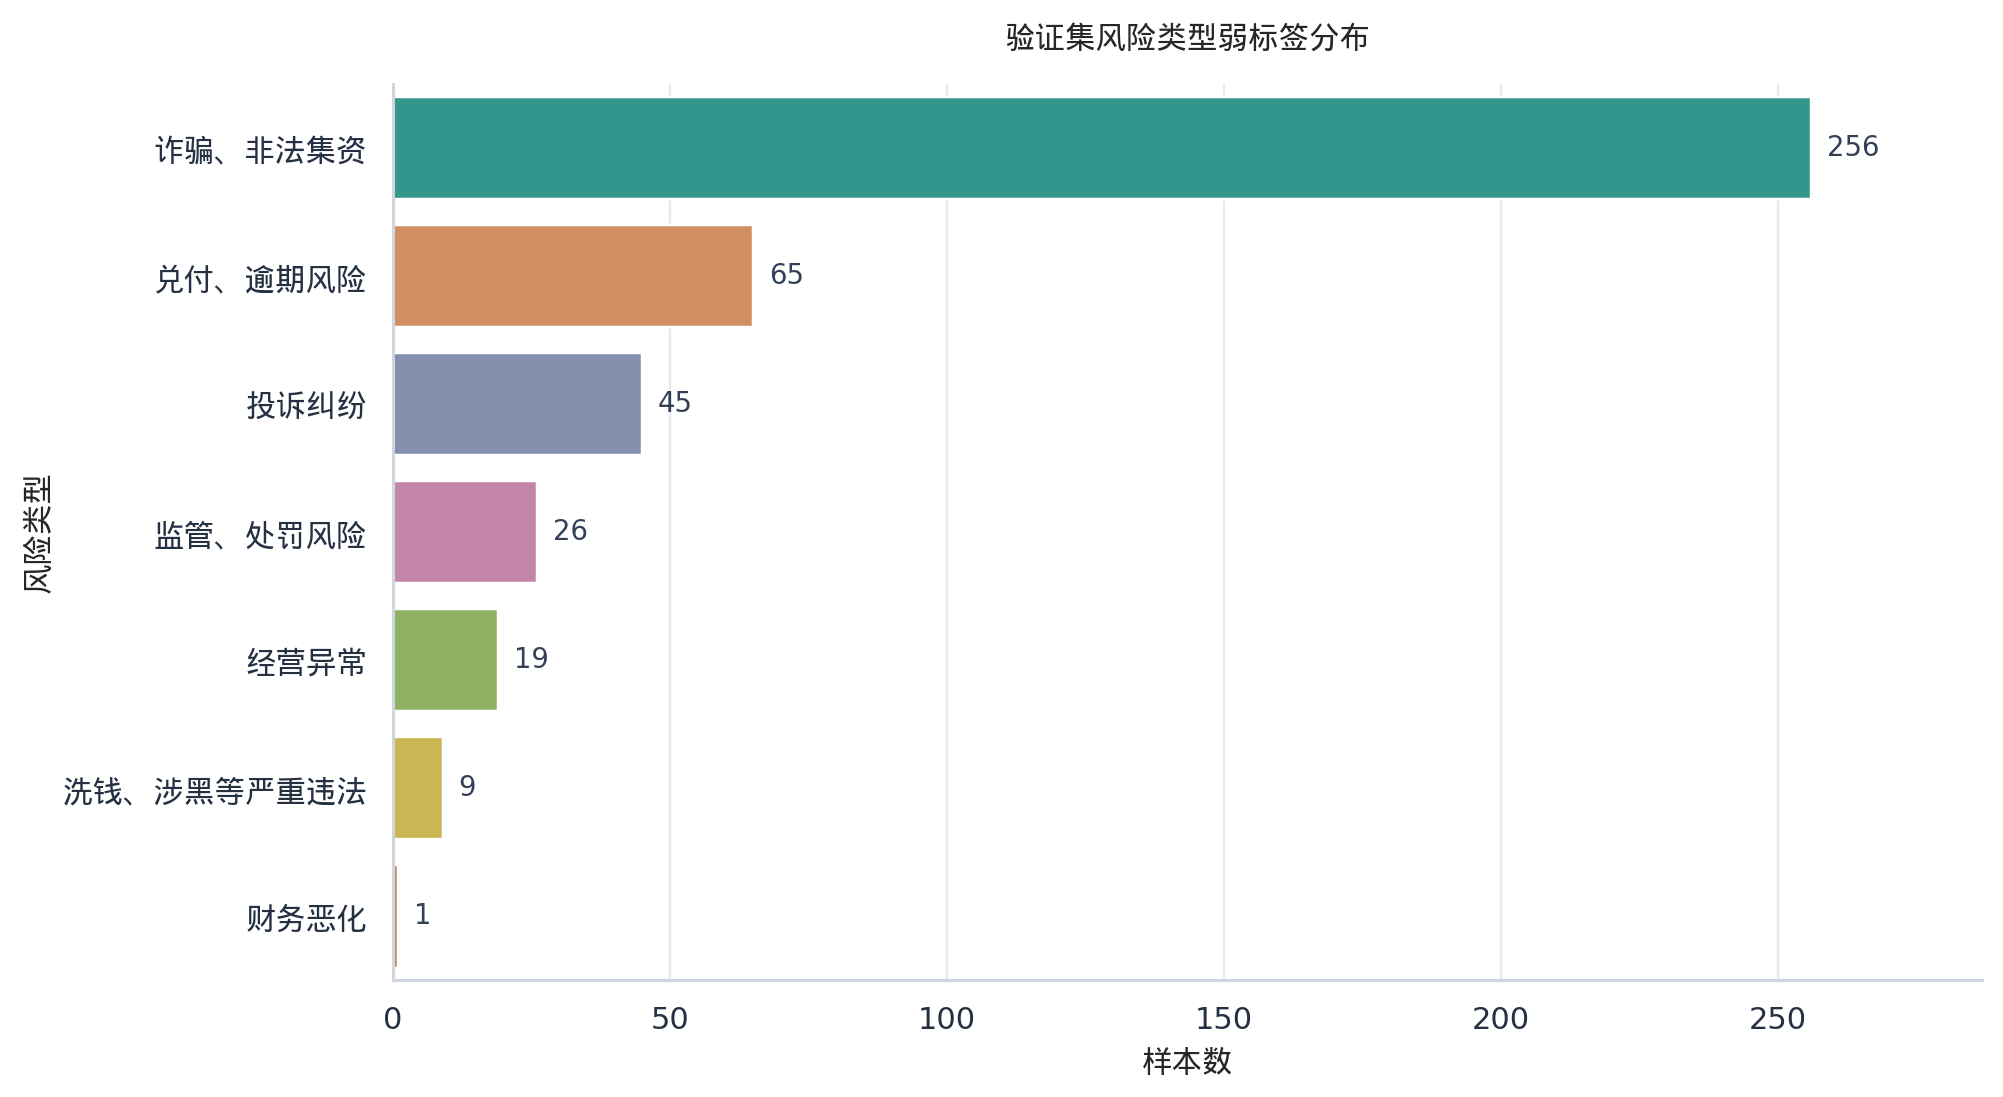
\includegraphics[width=\linewidth]{../outputs/figures/eval_risk_type_distribution.png}
    \caption{验证集风险类型弱标签}
  \end{subfigure}
  \caption{风险类型弱标签分布}
  \label{fig:risk_type_distribution}
\end{figure}

主体画像基于 FINNSP eval gold 弱标签构建，用于演示风险库能力。画像指标包括事件次数、最高风险等级、平均风险分、风险类型分布和最近证据。该部分属于演示库，不能夸大为线上长期自动沉淀的真实生产画像。

\subsection{外部扩展、反事实与 Tabular 风控}

除 FINNSP 主任务外，本文还补充三个扩展实验，用于观察模型迁移、扰动边界和结构化风控扩展能力。

第一，外部泛化评估使用 FLARE-zh-NSP 数据集的 500 条测试样本。关键词弱监督 baseline 的 F1 为 0.8808；将 Qwen3-8B QLoRA 主模型直接接入该外部集做真实推理后，二分类 Accuracy 为 0.9700、F1 为 0.9715、Macro-F1 为 0.9699，invalid JSON rate 为 0。这一结果表明主模型在同类外部金融负面判断任务上仍具有较好迁移能力。当前 FLARE-zh-NSP 处理流程只提供有/无二分类标签，缺少负面主体 gold，因此该外部实验只作为二分类泛化评估，不计算 Entity-F1。

第二，反事实样本构造覆盖主体替换、负面词删除、干扰主体插入和否定/澄清语境。该部分定位为自动构造压力测试，而不是主任务性能指标。Qwen3-8B QLoRA 在 400 条反事实样本上的实测结果显示，模型对干扰主体和否定/澄清语境较稳定，distractor resistance 为 0.9500，negation robustness 为 0.9400，invalid JSON rate 仍为 0；但主体替换和负面触发词删除两类扰动较困难，entity switch accuracy 为 0.4500，negative cue sensitivity 为 0.0400。原因在于，自动替换主体后，原文本中可能仍保留其他真实风险主体；删除少量显式负面词后，文本中也可能残留风险提示、备案异常等弱风险线索。因此，该实验主要用于揭示模型边界，而不作为主模型效果的核心结论。

第三，Tabular 风控分支使用 OpenML/UCI 真实信用卡违约数据集训练 LightGBM，报告 AUC、KS、PSI、Precision 和 Recall。该实验表明，文本舆情风险信号可以与传统结构化信用风险建模衔接；后续可将文本风险分数作为外部特征，与账单、还款、额度等变量融合，形成 hybrid risk 模型。

\subsection{漂移监控原型与上线讨论}

风控模型上线后需要持续监控数据分布和预测分布。本文实现的是轻量级离线漂移监控原型：以 FINNSP 训练集构造 baseline 快照，以验证集构造 current 快照，并结合主模型可靠性指标记录幻觉实体率和 invalid JSON rate。对于正例率、平均文本长度和平均实体数等标量指标，漂移量按式 \ref{eq:drift_delta} 计算。表 \ref{tab:drift_monitoring} 给出当前生成的漂移报告。

\begin{equation}
\Delta m=m_{\mathrm{current}}-m_{\mathrm{baseline}}.
\label{eq:drift_delta}
\end{equation}

\begin{table}[H]
\centering
\caption{离线漂移监控快照}
\label{tab:drift_monitoring}
\small
\begin{tabular}{lrrr}
\toprule
指标 & baseline & current & delta \\
\midrule
样本数 & 4000 & 500 & - \\
正例率 & 0.5447 & 0.5060 & -0.0387 \\
平均文本长度 & 224.6302 & 242.2900 & 17.6598 \\
平均实体数 & 0.9407 & 0.8420 & -0.0988 \\
幻觉实体率 & 不适用 & 0.0136 & - \\
invalid JSON rate & 不适用 & 0.0000 & - \\
\bottomrule
\end{tabular}
\end{table}

从当前快照看，验证集相对训练集的正例率下降 0.0387，平均文本长度增加 17.6598，平均实体数下降 0.0988，未触发按正例率阈值设置的重训建议。由于 baseline 来自训练集 gold 弱标签事件，不是模型在线预测日志，因此幻觉实体率和 invalid JSON rate 只在 current 侧统计。该实验应理解为监控字段和快照流程的原型验证，不等同于真实生产环境的时间序列漂移监控。若未来接入线上数据，还需要按日或按周聚合预测日志，补充分布距离、告警阈值、人工审核反馈和重训触发策略。

上线时应采用分层部署策略。高吞吐场景下，编码器模型负责全量初筛；LLM 只处理高风险、低置信度或需要主体归因的样本；人工审核处理高风险、主体缺失或实体不一致样本。这样可以在成本、召回率和可解释性之间取得平衡。

\subsection{当前不足与后续优化}

本文仍存在若干不足。首先，主体抽取仍依赖生成式模型和规则过滤，多主体文本中的边界错误较多，后续可引入金融 NER、实体链接和别名库，提高主体标准化能力。其次，风险类型和严重程度来自关键词弱标签，不是人工标注多分类任务，未来可以构建更细粒度的风险事件标注集。第三，外部泛化实验已完成二分类真实推理，但外部数据缺少实体级 gold，尚不能验证跨数据集主体抽取能力；反事实实测也表明，模型对干扰主体和澄清语境较稳，但对主体替换和负面词删除仍较敏感。第四，FastAPI 与 Streamlit 原型已经具备演示能力，但还缺少审核反馈闭环和再训练数据沉淀机制。

\section{结论}

本文围绕中文金融负面主体识别任务，构建了从模型实验到风控系统原型的技术路线。实验表明，Qwen3-8B QLoRA 在 FINNSP 验证集上取得 F1 0.9732 和 Entity-F1 0.8331，优于传统机器学习、通用中文编码器和金融领域编码器基线。相比普通二分类模型，QLoRA 主模型能够稳定输出 JSON 和负面主体，更适合金融风控中的实体级归因需求。离线级联模拟表明，FinBERT2-large 初筛与 Qwen3-8B QLoRA 复核可以在降低 LLM 调用率的同时保持较高效果。风险事件、风险评分、主体画像、审核队列、漂移监控和 tabular 风控扩展，则把课程实验推进到可演示的中文金融舆情风险智能预警系统原型。

\begin{thebibliography}{99}
\bibitem{bert} Devlin, J., Chang, M.-W., Lee, K., Toutanova, K. BERT: Pre-training of Deep Bidirectional Transformers for Language Understanding. NAACL, 2019. \url{https://arxiv.org/abs/1810.04805}
\bibitem{roberta} Liu, Y., Ott, M., Goyal, N., et al. RoBERTa: A Robustly Optimized BERT Pretraining Approach. 2019. \url{https://arxiv.org/abs/1907.11692}
\bibitem{macbert} Cui, Y., Che, W., Liu, T., Qin, B., Yang, Z. Revisiting Pre-Trained Models for Chinese Natural Language Processing. Findings of EMNLP, 2020. \url{https://arxiv.org/abs/2004.13922}
\bibitem{finbert} Araci, D. FinBERT: Financial Sentiment Analysis with Pre-trained Language Models. 2019. \url{https://arxiv.org/abs/1908.10063}
\bibitem{bbtfin} BBT-Fin / FinCUGE: A Chinese Financial Natural Language Processing Benchmark and Model. \url{https://huggingface.co/papers/2302.09432}
\bibitem{fincuge} FinCUGE-Instruction Dataset. \url{https://huggingface.co/datasets/Maciel/FinCUGE-Instruction}
\bibitem{flare} FLARE-zh-NSP Dataset. \url{https://huggingface.co/datasets/ChanceFocus/flare-zh-nsp}
\bibitem{bloomberggpt} Wu, S., Irsoy, O., Lu, S., et al. BloombergGPT: A Large Language Model for Finance. 2023. \url{https://arxiv.org/abs/2303.17564}
\bibitem{fingpt} AI4Finance Foundation. FinGPT: Open-Source Financial Large Language Models. \url{https://github.com/AI4Finance-Foundation/FinGPT}
\bibitem{pixiu} The FinAI. PIXIU / FinBen: Financial Large Language Model Benchmark. \url{https://github.com/The-FinAI/PIXIU}
\bibitem{lora} Hu, E. J., Shen, Y., Wallis, P., et al. LoRA: Low-Rank Adaptation of Large Language Models. ICLR, 2022. \url{https://arxiv.org/abs/2106.09685}
\bibitem{qlora} Dettmers, T., Pagnoni, A., Holtzman, A., Zettlemoyer, L. QLoRA: Efficient Finetuning of Quantized LLMs. NeurIPS, 2023. \url{https://arxiv.org/abs/2305.14314}
\end{thebibliography}

\end{document}
